% To generate PDF, type ./run approximate

\documentclass{article}
\usepackage{arxiv}
\usepackage[numbers]{natbib} % for author-year citation style: \usepackage{natbib}
\numberwithin{equation}{section} % numbering of equations as 2.1 (for section 2, equation 1)

\newcommand{\mat}[1]{\mathbf{#1}}          % shortcut for matrix
\newcommand{\dpro}[1]{\langle #1 \rangle}  % shortcut for dot-product

% shortcuts for matrices Q, K, V, O and vectors q, k, v, o, t, u
\def\Q{\mat{Q}}
\def\K{\mat{K}}
\def\V{\mat{V}}
\def\O{\mat{O}}
\def\q{\vec{q}}
\def\k{\vec{k}}
\def\v{\vec{v}}
\def\o{\vec{o}}
\def\t{\vec{t}}
\def\u{\vec{u}}

% more shortcuts
\def\dotqk{\dpro{\q, \k_i}}  % dot-product between vectors q and k_i
\def\edotqk{\exp(\dotqk)}    % exponent of dot-product between vectors q and k_i

%\title{Transformer tricks: Approximate attention [work in progress]}
\title{Approximate attention: infinite context length with constant complexity per token [work in progress]}

\author{Nils Graef, Aarush Gupta, TBD \\ \href{https://openmachine.ai}{OpenMachine},
  San Francisco Bay Area, \texttt{info@openmachine.ai}}

\begin{document} \maketitle

\begin{abstract}
This micro-paper \citep{micro-paper} details a hybrid between exact and approximate dot-product attention for transformers that use rotary position embedding (RoPE) \citep{RoPE} (such as LLaMA, Mistral, and Gemma \citep{LLaMA, Llama2, mistral, gemma}). The approximation is done by polynomials. For polynomial degree 1, this scheme is a hybrid between local attention \citep{longformer} and linear transformer \citep{linear}. The goal is to reduce the computational complexity and memory size of attention for a given LLM without changing its weights (especially for long context lengths). See \citep{tricks, precompute} for code and more transformer tricks.
\end{abstract}

\section{Scaled dot-product attention}
Recall that the scaled dot-product attention of the vanilla transformer \citep{vanilla} is defined as
\begin{equation}
  \O = \text{Attention} \left( \Q, \K, \V \right) = \text{softmax} \left( \frac{\Q \K^T}{\sqrt{d_k}} \right) \V
\end{equation}

with the following variables:
\begin{itemize}[topsep=-1pt, itemsep=-1pt]
  \item $d_k$ is the dimension of keys and queries; $d_v$ is the dimension of values.
  \item $s$ is the current sequence length (aka context length).
  \item $\Q$ and $\K$ are matrices of dimension $s \times d_k$. $\V$ and output $\O$ are $s \times d_v$ matrices.
\end{itemize}

Let’s make the following assumptions:
\begin{itemize}[topsep=-1pt, itemsep=-1pt]
  \item For simplicity, we assume that $d = d_k = d_v$, which is the case for many popular LLMs.
  \item At the output of the transformer decoder stack, we only need to compute the last token of the output matrix $\O$, i.e. the last row of $\O$, which is the $d$-dimensional vector $\o$. Therefore, during the autoregressive next-token-generation process, we only need to compute the last row of $\O$ for each layer of the transformer stack.
  \item Similarly, we only need the last row of $\Q$, which is the $d$-dimensional vector $\q$.
  \item We also need matrices $\K$ and $\V$, which we organize (in a KV-cache) as $s$ pairs of KV-vectors called $\k_i$ and $\v_i$.
  \item Furthermore, we assume that the scaling factor $1/\sqrt{d}$ is already merged into $\q_i$ or $\k_i$. For example, this scaling factor could be included into the weights (and biases) of the linear layer K by scaling its weights (and biases) by $1/\sqrt{d}$.
\end{itemize}

We can now express the output vector $\o$ as follows, where $\dpro{.}$ denotes the dot-product:
\begin{equation}
  \o = \sum_{i = 1}^s \text{softmax}(\dotqk) \v_i
     = \sum_{i = 1}^s \frac{\edotqk}{\sum_{i = 1}^s \edotqk} \v_i
\label{eq1.2} \end{equation}

\section{Hybrid between exact and approximate attention with RoPE}
RoPE is used by many popular LLMs such as LLaMA and Mistral. RoPE modifies the vectors $\q$ and $\k$, which results in scaling of the dot-products. This dot-product scaling decays with the relative distance between keys as illustrated in Figure \ref{fig1}, which is copied from the RoPE paper \citep{RoPE}.

For example, only the 200 most recent keys have high scaling factors (closer to 1) while the older keys have scaling closer to 0. Therefore, we can split the key-value pairs (KV-pairs) into the following two groups, where $N$ is 200 for example and $g = s - N$ is a shortcut variable:
\begingroup \renewcommand{\arraystretch}{1.3} % increase table row height by 1.3x
\begin{center} \begin{tabular}{c|c|c|c|c}
  \textbf{Group} & \textbf{KV-pairs} & \textbf{Index range} & \textbf{Dot-product magnitudes} & \textbf{Calculation of exp(x)} \\ \hline
  1 & $N$ most recent      & $i = (g + 1), .., s$ & large                   & exact                    \\ \hline
  2 & older than $N$ steps & $i = 1, .., g$       & small (e.g. [-1 .. +1]) & polynomial approximation
\end{tabular} \end{center} \endgroup

Specifically, the first group contains the $N$ most recent key-value pairs, and the second group contains the remaining $g$ pairs. The $N$ most recent KV-pairs (first group) are processed explicitly, while the remaining $g$ KV-pairs are used for polynomial approximation. Derived from equation (\ref{eq1.2}), below equation shows how this hybrid scheme combines these two groups:
\begin{equation}
  \o = \sum_{i = 1}^s \frac{\edotqk}{\sum_{i = 1}^s \edotqk} \v_i
     = \left(\sum_{i=g+1}^s \edotqk \v_i + \sum_{i=1}^g \edotqk \v_i \right)
       \frac{1}{D_1 + D_2} = \frac{\t + \u}{D_1 + D_2}
\label{eq2.1} \end{equation}
where
\begin{align} \begin{split}
  \t  &= \sum_{i=g+1}^s \edotqk \v_i \\
  D_1 &= \sum_{i=g+1}^s \edotqk \\
  \u  &= \sum_{i=1}^g   \edotqk \v_i \\
  D_2 &= \sum_{i=1}^g   \edotqk
\label{eq2.2} \end{split} \end{align}

We can now compute vector $\t$ of equation (\ref{eq2.2}) explicitly using the $\exp(x)$ function. And vector $\u$ can be approximated by polynomials. Note that the exact softmax attention is only calculated for the $N$ first KV-pairs (e.g. $N = 200$), which reduces the size of the KV-cache to only  200 KV-pairs irrespectively of the actual context length $s$. The calculation of $\t$ is similar (or identical) to the sliding window attention (SWA) \citep{longformer}. However, here we can set the window length to a smaller value (e.g. 200 instead of 4096 as used in Mistral-7B).

If the approximate attention uses a polynomial degree of 1, then this scheme is a hybrid of SWA (aka local attention) and linear attention \citep{linear} (which can be considered as a recurrent network \citep{linear}). Griffin \citep{griffin} also mixes recurrences with local attention. However, here we only modify the attention mechanism (see Figure \ref{fig2}) without changing any weights. Our goal is post-training approximation of a given transformer without chaging its weights.

\begin{figure}[h!] \centering  % the [h!] tries to place the picture right here
  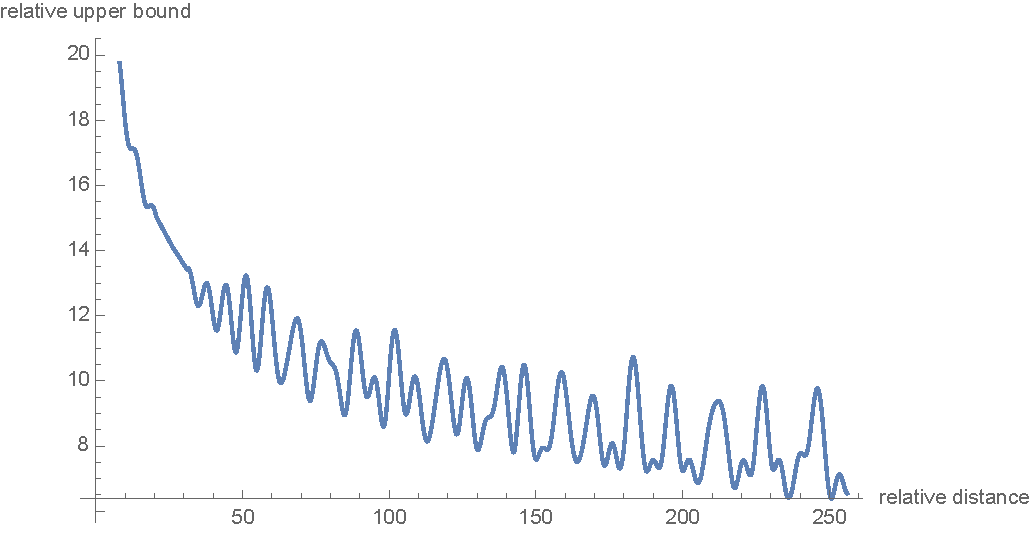
\includegraphics[scale=0.76]{figs/approximate_fig1.pdf}
  \caption{Long-term decay of RoPE, copied from \citep{RoPE}}
\label{fig1} \end{figure}

\textbf{Better numerical stability}.  For higher numerical stability, many softmax implementations such as flash attention \citep{flash-attention} subtract the maximum $m$ across all softmax-arguments so that the arguments $x$ of $\exp(x)$ are $x \leq 0$, and thus $\exp(x)$ is between 0 and 1. After subtracting the maximum $m$ from the softmax arguments, we get $\t^*$ and $D_1^*$ (instead of $\t$ and $D_1$) as follows (note that $e^{-m}$ is identical to $\exp(-m)$):
\begin{align} \begin{split}
  \t^*  &= \sum_{i=g+1}^s \exp(\dotqk -m) \v_i = e^{-m} \cdot \t \\
  D_1^* &= \sum_{i=g+1}^s \exp(\dotqk -m)      = e^{-m} \cdot D_1
\end{split} \end{align}

We can now calculate output vector $\o$ by scaling $\u$ and $D_2$ by the same scaling factor $e^{-m}$ as
\begin{equation}
  \o = \frac{e^{-m} (\t + \u)}{e^{-m} (D_1 + D_2)} = \frac{\t^* + e^{-m} \u}{D_1^* + e^{-m} D_2}
\label{eq2.4} \end{equation}

\textbf{Block diagram}. Figure \ref{fig2} shows an implementation of this hybrid scheme:
\begin{itemize}[topsep=-1pt, itemsep=-1pt]
  \item The block labeled SWA (sliding window attention) consists of a sliding window KV-cache of depth $N$ (implemented by a circular buffer) followed by “exact attention.”
  \item The “exact attention” block calculates vector $\t$ from the $N$ KV-pairs it receives from the KV-cache and from the latest query vector $\q_s$ (e.g. by using flash attention \citep{flash-attention}). If the sequence length $s$ is smaller than $N$, then it only processes $s$ KV-pairs.
  \item The “approximate attention” block receives the $N$-th KV-pair from the KV-cache if $s$ is greater than or equal to $N$. The approximate attention block uses this KV-pair and the latest query vector $\q_s$ to approximate $\u$ and $D_2$.
  \item Note that the query and key vectors ($\q$ and $\k$) shown in the figure already include the rotations performed by RoPE.
  \item Finally, adders and multipliers are used to compute the output vector $\o$ according to equation (\ref{eq2.4}).
\end{itemize}

\begin{figure}[h!] \centering  % the [h!] tries to place the picture right here
  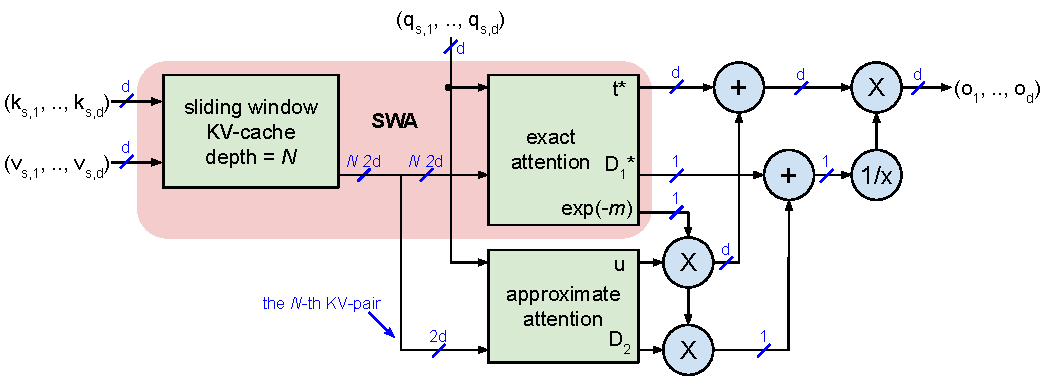
\includegraphics[scale=0.86]{figs/approximate_fig2.pdf}
  \caption{Block diagram of hybrid between exact and approximate attention}
\label{fig2} \end{figure}

The rest of this paper details the polynomial approximation of $\u$ and $D_2$.

\section{Polynomial approximation of $\exp(x)$}
In general, the exponential function can be approximated by a polynomial of degree $n$ as follows:
\begin{equation}
  \exp(x) \approx a_0 + a_1 x + a_2 x^2 + \cdots + a_n x^n
\end{equation}

Many computers (or maybe all computers) implement the floating-point exponential function by a combination of argument-reduction and polynomial approximation over a small range, see \citep{exp.c} for example.

The polynomial coefficinets $a_i$ can be calculated by using Taylor, Chebyshev \citep{chebyshev}, or minimax approximation algorithms \citep{minimax}. The polynomial approximation of $\exp(x)$ is only accurate for a small range, e.g. only for $x = -1 \ldots 1$. If $x$ falls outside this range, then the approximation error becomes large. Even worse, the polynomial might not be monotonic outside this range, which violates a key requirement for softmax to work properly as a way to generate a probability distribution. For the Taylor approximation, the table below lists the absolute and relative errors for polynomial degrees $n = 1$ to 4 for various values of $x$.

\begingroup \renewcommand{\arraystretch}{1.1} % increase table row height by 1.1x
\begin{center} \begin{tabular}{c|c|c|c|c|c|c|c|c|c}
  & & \multicolumn{2}{c|}{error for $n=1$} & \multicolumn{2}{c|}{error for $n=2$}
    & \multicolumn{2}{c|}{error for $n=3$} & \multicolumn{2}{c} {error for $n=4$} \\
  $x$  & $\exp(x)$ & abs. & rel.    & abs.  & rel      . & abs. & rel.       & abs. & rel. \\ \hline
  0.25 &  1.28 &  0.03 &\textbf{3\%}&  0.00 &\textbf{0\%}& 0.00 &\textbf{0\%}& 0.00 &\textbf{0\%} \\
  0.5  &  1.65 &  0.15 &        9\% &  0.02 &\textbf{1\%}& 0.00 &\textbf{0\%}& 0.00 &\textbf{0\%} \\
  1.0  &  2.72 &  0.72 &       26\% &  0.22 &        8\% & 0.05 &\textbf{2\%}& 0.01 &\textbf{0\%} \\
  1.5  &  4.48 &  1.98 &       44\% &  0.86 &       19\% & 0.29 &        7\% & 0.08 &\textbf{2\%} \\
  2.0  &  7.39 &  4.39 &       59\% &  2.39 &       32\% & 1.06 &       14\% & 0.39 &        5\%  \\
  2.5  & 12.18 &  8.68 &       71\% &  5.56 &       46\% & 2.95 &       24\% & 1.33 &       11\%  \\
  3.0  & 20.09 & 16.09 &       80\% & 11.59 &       58\% & 7.09 &       35\% & 3.71 &       18\%
\end{tabular} \end{center} \endgroup

The scaling factor $1/\sqrt{d}$ helps to reduce the range of the dot-product. As mentioned in the previous section, RoPE essentially scales down dot-products with increasing distance. And the recently proposed “clipped softmax” \citep{quantizable} is another method that limits the range of dot-products, especially for outliers that are often correlated with delimiter tokens such as [SEP], “.”, and “,” \citep{quantizable}.

\section{Approximation for case $d = 2$ with quadratic polynomial}
For simplicity, let’s assume that $d = 2$ and we approximate the exponential function by a polynomial of degree two (with coefficients $a_0 = a, a_1 = b, a_2 = c$) as follows:
\begin{equation}
  \exp(x) \approx a + b x + c x^2
\label{eq4.1} \end{equation}

Let’s plug the two-dimensional dot-product $\dotqk = q_1 k_{i,1} + q_2 k_{i,2}$ into equation (\ref{eq4.1}):
\begin{equation}
  \exp(q_1 k_{i,1} + q_2 k_{i,2}) \approx a + b (q_1 k_{i,1} + q_2 k_{i,2}) + c (q_1 k_{i,1} + q_2 k_{i,2})^2
\end{equation}
Plugging above into equation (\ref{eq2.2}) yields
\begin{align} \begin{split}
  \u  &\approx \sum_{i=1}^g \left(a + b (q_1 k_{i,1} + q_2 k_{i,2}) + c (q_1 k_{i,1} + q_2 k_{i,2})^2 \right) \v_i \\
  D_2 &\approx \sum_{i=1}^g       a + b (q_1 k_{i,1} + q_2 k_{i,2}) + c (q_1 k_{i,1} + q_2 k_{i,2})^2
\label{eq4.3} \end{split} \end{align}

Similar to the linear transformer \citep{linear}, we can now expand equation (\ref{eq4.3}) as follows
\begin{align} \begin{split}
  \u  &\approx a \sum_{i=1}^g \v_i + b q_1 \sum_{i=1}^g k_{i,1} \v_i + b q_2 \sum_{i=1}^g k_{i,2} \v_i
        + c q_1^2 \sum_{i=1}^g k_{i,1}^2 \v_i + 2c q_1 q_2 \sum_{i=1}^g k_{i,1} k_{i,2} \v_i
        + c q_2^2 \sum_{i=1}^g k_{i,2}^2 \v_i \\
  D_2 &\approx a g + b q_1 \sum_{i=1}^g k_{i,1} + b q_2 \sum_{i=1}^g k_{i,2}
        + c q_1^2 \sum_{i=1}^g k_{i,1}^2 + 2c q_1 q_2 \sum_{i=1}^g k_{i,1} k_{i,2}
        + c q_2^2 \sum_{i=1}^g k_{i,2}^2
\label{eq4.4} \end{split} \end{align}

As was already shown in the linear transformer paper \citep{linear}, the advantages of equation (\ref{eq4.4}) include lower memory and computational complexities:
\begin{itemize}[topsep=-1pt, itemsep=-1pt]
  \item We don’t need to store the $g$ KV-pairs anymore. Instead, we only need to store the sum terms such as $\sum_{i=1}^g k_{i,1} \v_i$, which we update in each iteration of the autoregressive next-token-generation process. Specifically, for $d = 2$ and quadratic polynomial approximation, we only need to store 6 KV-sums (each such sum-vector has dimension 2) and 5 sums (or sum-scalars) for the denominator $D_2$. So in total, we only need to store 12 + 5 = 17 values. Let’s call this storage “KV-state” (as opposed to KV-cache).
  \item This also reduces the computational complexity significantly.
  \item More importantly, the memory size for the KV-state is constant; and the computational complexity per token is constant, too. Specifically, memory size and compute complexity per token are independent from the current sequence length $s$, which allows us to support infinitely long sequences.
  \item Furthermore, for applications where you want to store a conversation history (e.g. for a personal assistant or an AI companion), it would be more efficient (in terms of compute and perhaps also memory) to store the KV-state of that conversation history instead of storing and reprocessing a very long input sequence of tokens.
\end{itemize}

Figures \ref{fig3} and \ref{fig4} show block diagrams to approximate the output vector $\u$ and denominator $D_2$ according to equation (\ref{eq4.4}). There are two steps:
\begin{itemize}[topsep=-1pt, itemsep=-1pt]
  \item Step 1: Update the KV-state, i.e. all KV-sums (or sum-vectors and sum-scalars).
  \item Step 2: Calculate the output-vector $\u$ and denominator $D_2$ by multiplying elements of $\q$ with the KV-sums.
\end{itemize}

The blocks labeled “reg” in the figures denote registers that hold the KV-state. These registers, together with their preceding adders, form accumulators to implement the sums of equation (\ref{eq4.4}). Alternatively, the KV-state can be implemented in SRAM or off-chip DRAM.

\begin{figure}[h!] \centering  % the [h!] tries to place the picture right here
  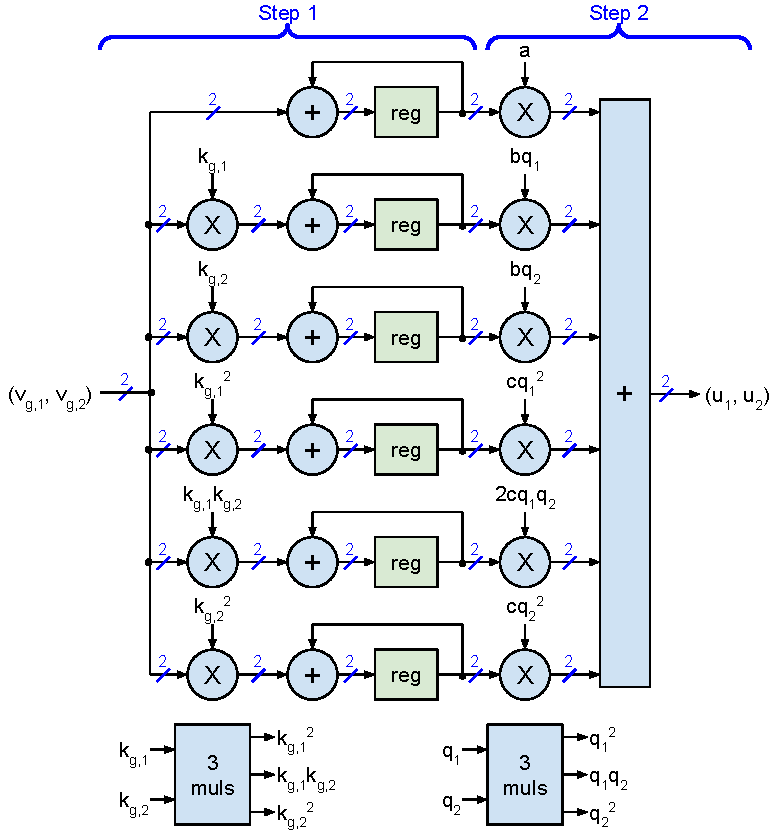
\includegraphics[scale=0.86]{figs/approximate_fig3.pdf}
  \caption{Block diagram for approximating vector $\u$ for $d=2$}
\label{fig3} \end{figure}

\begin{figure} \centering
  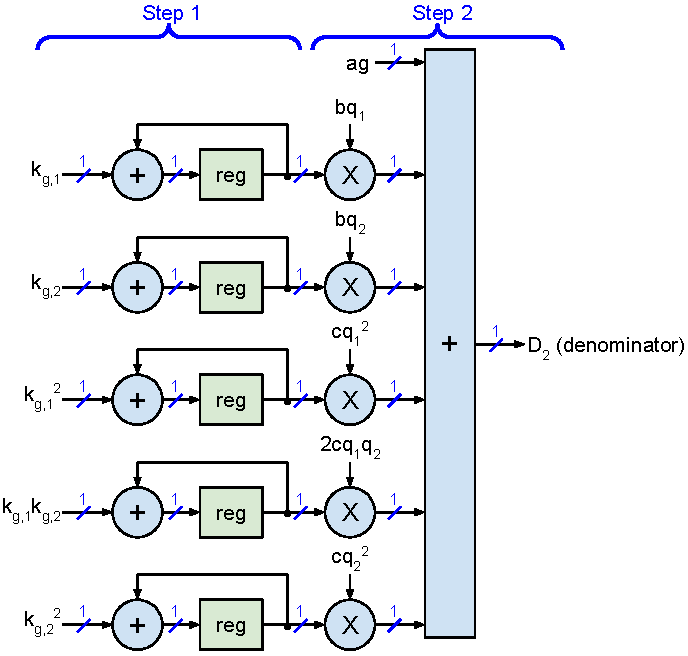
\includegraphics[scale=0.86]{figs/approximate_fig4.pdf}
  \caption{Block diagram for approximating denominator $D_2$ for $d=2$}
\label{fig4} \end{figure}

\section{General case}
The two-dimensional example ($d = 2$) is not very realistic: Many LLMs use $d = 64, 128$, or $256$. Therefore, the equations for arbitrary dimension $d$ and arbitrary polynomial degree $n$ are given in this section.

\subsection{Arbitrary $d$ with quadratic polynomial}
Let’s plug the $d$-dimensional dot-product $\dotqk$ into equation (\ref{eq4.1}):
\begin{equation}
  \exp \left( \sum_{j=1}^d \q_j \k_{i,j} \right) \approx a + b \sum_{j=1}^d \q_j \k_{i,j} + c \left( \sum_{j=1}^d \q_j \k_{i,j} \right)^2
\label{eq5.1} \end{equation}

Note that the last term of equation (\ref{eq5.1}) can be expanded to $1+2+...+d$ terms, i.e. $\sum_{i=1}^d i = \frac{d(d+1)}{2}$ terms, as follows
\begin{equation*}
  \left( \sum_{j=1}^d \q_j \k_j \right)^2 = q_1^2 k_1^2 + 2 q_1 q_2 k_1 k_2 + \cdots + 2 q_1 q_d k_1 k_d + q_2^2 k_2^2
  + 2 q_2 q_3 k_2 k_3 + \cdots + 2 q_2 q_d k_2 k_d + \cdots + q_d^2 k_d^2
\end{equation*}

which we will shorten as follows for use in equation (\ref{eq5.3}) below:
\begin{equation*}
  \left( \sum_{j=1}^d \q_j \k_j \right)^2 = q_1^2 k_1^2 + 2 q_1 q_2 k_1 k_2 + \cdots + q_d^2 k_d^2
\end{equation*}

Plugging equation (\ref{eq5.1}) into equation (\ref{eq2.2}) yields
\begin{align} \begin{split}
  \u   &\approx \sum_{i=1}^g \left[ a + b \sum_{j=1}^d \q_j \k_{i,j} + c \left( \sum_{j=1}^d \q_j \k_{i,j} \right)^2 \right] \v_i \\
  D_2  &\approx \sum_{i=1}^g \left[ a + b \sum_{j=1}^d \q_j \k_{i,j} + c \left( \sum_{j=1}^d \q_j \k_{i,j} \right)^2 \right]
\label{eq5.2} \end{split} \end{align}

We can now expand equation (\ref{eq5.2}) as follows
\begin{align} \begin{split}
  \u  &\approx a \sum_{i=1}^g \v_i + b q_1 \sum_{i=1}^g k_{i,1} \v_i + \cdots
  + b q_d \sum_{i=1}^g k_{i,d} \v_i + c q_1^2 \sum_{i=1}^g k_{i,1}^2 \v_i
  + 2c q_1 q_2 \sum_{i=1}^g k_{i,1} k_{i,2} \v_i + \cdots
  + c q_d^2 \sum_{i=1}^g k_{i,d}^2 \v_i \\
  D_2 &\approx a g + b q_1 \sum_{i=1}^g k_{i,1} + \cdots
  + b q_d \sum_{i=1}^g k_{i,d} + c q_1^2 \sum_{i=1}^g k_{i,1}^2
  + 2 c q_1 q_2 \sum_{i=1}^g k_{i,1} k_{i,2} + \cdots
  + c q_d^2 \sum_{i=1}^g k_{i,d}^2
\label{eq5.3} \end{split} \end{align}

The total number of KV-sums of equation (\ref{eq5.3}) is $1 + d + \frac{d(d+1)}{2}$.

\begin{figure}[h!] \centering  % the [h!] tries to place the picture right here
  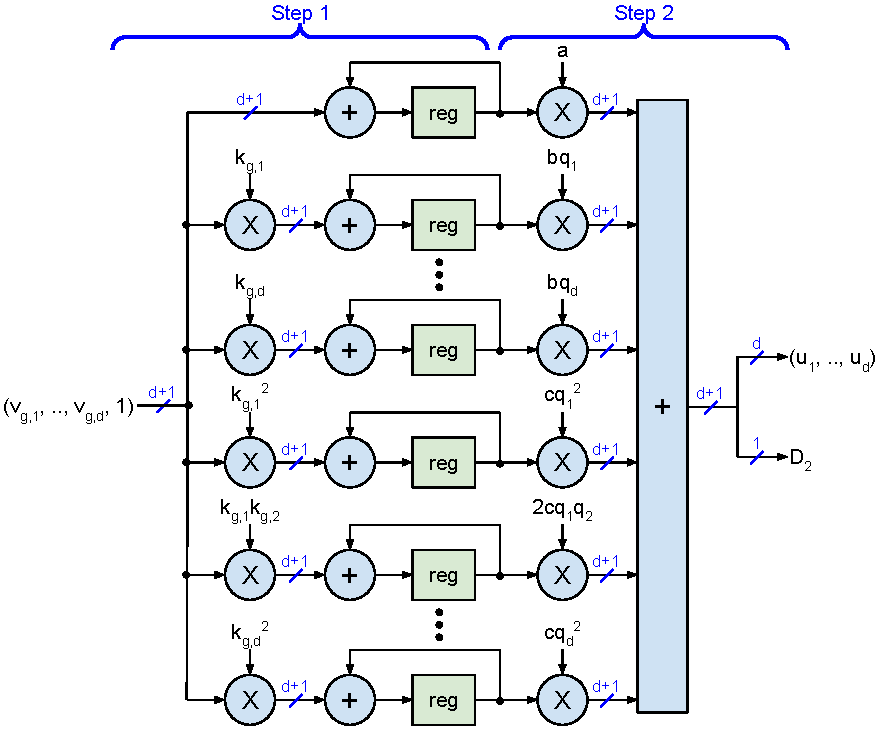
\includegraphics[scale=0.86]{figs/approximate_fig5.pdf}
  \caption{Block diagram for approximating vector $\u$ and denominator $D_2$}
\label{fig5} \end{figure}

Figure \ref{fig5} shows an implementation that approximates the output vector $\u$ and denominator $D_2$ according to equation (\ref{eq5.3}): The arithmetic blocks for $\u$ and $D_2$ are merged into one block diagram by appending a constant 1 to the input vector $(v_{g,1}, .., v_{g,d})$ to form a new vector $(v_{g,1}, ..,v_{g,d}, 1)$. This constant 1 is used for computing the denominator $D_2$.

\subsection{Arbitrary $d$ with cubic polynomial ($n = 3$)}
Let’s plug the $d$-dimensional dot-product $\dotqk$ into equation (\ref{eq4.1}) and let’s add a cubic term with the polynomial coefficient $e$ as follows
\begin{equation}
  \exp \left( \sum_{j=1}^d \q_j \k_{i,j} \right) \approx a + b \sum_{j=1}^d \q_j \k_{i,j}
  + c \left( \sum_{j=1}^d \q_j \k_{i,j} \right)^2
  + e \left( \sum_{j=1}^d \q_j \k_{i,j} \right)^3
\label{eq5.4} \end{equation}

Plugging equation (\ref{eq5.4}) into equation (\ref{eq2.2}) yields
\begin{align} \begin{split}
  \u  &\approx \sum_{i=1}^g \left[ a + b \sum_{j=1}^d \q_j \k_{i,j}
    + c \left( \sum_{j=1}^d \q_j \k_{i,j} \right)^2
    + e \left( \sum_{j=1}^d \q_j \k_{i,j} \right)^3 \right] \v_i \\
  D_2 &\approx \sum_{i=1}^g \left[ a + b \sum_{j=1}^d \q_j \k_{i,j}
    + c \left( \sum_{j=1}^d \q_j \k_{i,j} \right)^2
    + e \left( \sum_{j=1}^d \q_j \k_{i,j} \right)^3 \right]
\label{eq5.5} \end{split} \end{align}

Similar to equation (\ref{eq4.4}), expanding equation (\ref{eq5.5}) yields a series of KV-sums. To determine the total number of KV-sums, we use the multinomial theorem \citep{multinomial}, which lets us expand a sum with $d$ terms raised to the $n$-th power as follows:
\begin{equation}
  (x_1 + x_2 + \cdots + x_d)^n = \sum_{k_1 + k_2 + \cdots + k_d = n; k_1, k_2, \ldots, k_d \ge 0}
    \binom{n}{k_1, k_2, \ldots, k_d} \prod_{t=1}^d x_t^{k_t}
\label{eq5.6} \end{equation}

where $\binom{n}{k_1, k_2, \ldots, k_d} = \frac{n!}{k_1! k_2! \cdots k_d!}$ is the multinomial coefficient. As stated in \citep{multinomial}, “the sum is taken over all combinations of nonnegative integer indices $k_1$ through $k_d$ such that the sum of all $k_i$ is $n$.” Furthermore, \citep{multinomial} gives the number of terms in a multinomial sum, $\#_{n,d}$, as
\begin{equation}
  \#_{n,d} = \binom{d+n-1}{d-1}
\label{eq5.7} \end{equation}

With $n = 3$, we get $\#_{n=3, d} = \binom{d+2}{d-1} = \frac{(d+2)!}{(d-1)! 3!} = \frac{d(d+1)(d+2)}{3!} = \frac{d (d+1) (d+2)}{6}$.
Note that this number of terms is in addition to the terms we already have for linear and quadratic. So the total number of KV-sums is
\begin{equation}
  \#_{total, n=3} = 1 + d + \frac{d(d+1)}{2} + \frac{d(d+1)(d+2)}{6}
\label{eq5.8} \end{equation}

\subsection{Arbitrary $d$ with arbitrary polynomial degree $n$}
The previous sections can be extended to polynomials of degree four and higher. We only give the number of KV-sums needed for this. Per equation (\ref{eq5.7}), the additional number of terms for degree $n$ is given as
\begin{equation}
  \#_{n, d} = \binom{d+n-1}{d-1} = \frac{(d+n-1)!}{(d-1)! n!} = \frac{1}{n!} \prod_{i=d}^{d+n-1} i = \frac{d (d+1) (d+2) \cdots (d+n-1)}{n!}
\label{eq5.9} \end{equation}

So the total number of KV-sums is:
\begin{equation}
  \#_{total} = 1 + \sum_{j=1}^n \left( \frac{1}{j!} \prod_{i=d}^{d+j-1} i \right)
  = 1 + d + \frac{d(d+1)}{2} + \frac{d(d+1)(d+2)}{6} + \cdots
  + \frac{d(d+1)(d+2) \cdots (d+n-1)}{n!}
\label{eq5.10} \end{equation}

\subsection{Sharing KV-pairs}
Many LLMs use multi-query attention (MQA) \citep{MQA} or grouped-query attention (GQA) \citep{GQA}, which reduces the size of the KV-cache significantly. It also reduces the sizes of the linear layers K and V, which reduces their computational complexity and weight storage size.
The same savings are also applicable to the polynomial approximation scheme detailed here. Specifically, for MQA, one set of KV-state is shared among all heads (or group of heads for GQA). Additionally, we can also share the computations needed for step 1 (i.e. for updating the KV-state) among all heads (or group of heads).

\section{Splitting dot-products into partial products}
This section details a way to reduce the required range of the polynomial approximation: We can split the dot-product into two or more partial products and then approximate each partial product by a lower-degree polynomial.

\subsection{Case $d = 2$ with two partial products and linear approximation}
Let’s first consider the simple case with $d = 2$ where we split the dot-product into two partial products and approximate each by a linear polynomial as

\begin{equation}
  \exp(q_1 k_{i,1} + q_2 k_{i,2}) = \exp(q_1 k_{i,1}) \cdot exp(q_2 k_{i,2})
  \approx (a + b q_1 k_{i,1}) (a + b q_2 k_{i,2})
\end{equation}

Plugging above into equation (\ref{eq2.2}) yields
\begin{align} \begin{split}
  \u  &\approx \sum_{i=1}^g (a + b q_1 k_{i,1}) (a + b q_2 k_{i,2}) \v_i \\
  D_2 &\approx \sum_{i=1}^g (a + b q_1 k_{i,1}) (a + b q_2 k_{i,2})
\label{eq6.2} \end{split} \end{align}

We can now expand equation (\ref{eq6.2}) as follows
\begin{align} \begin{split}
  \u  &\approx a^2 \sum_{i=1}^g \v_i
           + abq_1 \sum_{i=1}^g k_{i,1} \v_i
           + abq_2 \sum_{i=1}^g k_{i,2} \v_i
     + b^2 q_1 q_2 \sum_{i=1}^g k_{i,1} k_{i,2} \v_i \\
  D_2 &\approx a^2 g
           + abq_1 \sum_{i=1}^g k_{i,1}
           + abq_2 \sum_{i=1}^g k_{i,2}
     + b^2 q_1 q_2 \sum_{i=1}^g k_{i,1} k_{i,2}
\label{eq6.3} \end{split} \end{align}

Figure \ref{fig6} shows a block diagram that approximates the vector $\u$ and denominator $D_2$ according to equation (\ref{eq6.3}).

\begin{figure}[h!] \centering  % the [h!] tries to place the picture right here
  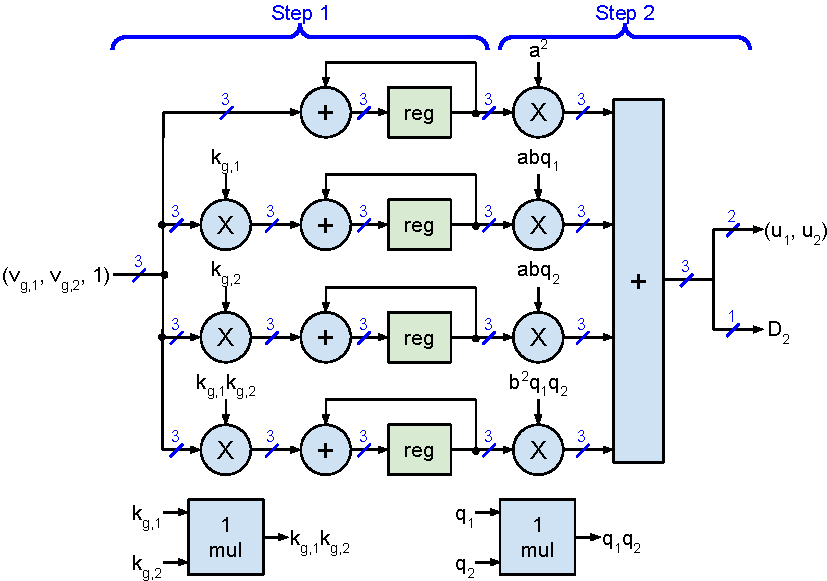
\includegraphics[scale=0.86]{figs/approximate_fig6.pdf}
  \caption{Block diagram for approximating vector $\u$ and denominator $D_2$ with two partial products for $d = 2$}
\label{fig6} \end{figure}

\subsection{General case and examples}
This section derives $\#_{total}$ (the number of KV-sums) for arbitrary dimension $d$, number of partitions $p$, and polynomial degree $n$:
\begin{itemize}[topsep=-1pt, itemsep=-1pt]
  \item \textbf{Polynomial degree $n = 1$} (i.e. we approximate each partition by a linear polynomial): In this case, the number of KV-sums is $\#_{total, n=1} = (1+ \frac{d}{p})^p$.
  \item \textbf{Polynomial degree $n = 2$} (i.e. we approximate each partition by a quadratic polynomial):
In this case, the total number of KV-sums is $\#_{total, n=2} = (1 + \frac{d}{p} + \frac{d/p(d/p+1)}{2})^p$.
  \item \textbf{Arbitrary polynomial degree $n$}: In this general case, the total number of KV-sums equals equation (\ref{eq5.10}) raised to the $p$-th power and where $d$ is replaced by $d/p$ as
\end{itemize}

\begin{equation}
  \#_{total} = \left(1 + \sum_{j=1}^n \left(\frac{1}{j!} \prod_{i=d/p}^{d/p +j-1} i \right) \right)^p
\end{equation}

For dimensions $d = 4, 8, 16, 32, 64, 128$, and $256$, the table below lists a few examples for $p$ and $n$.

\begingroup \renewcommand{\arraystretch}{1.3} % increase table row height by 1.3x
\quad \quad \quad
\begin{tabular}{c|c|c|r}
  $d$                & $p$              & $n$ & $\#_{total}$ \\ \hline
  \multirow{9}{*}{4} & \multirow{3}{*}{1} & 1 &   5 \\
                     &                    & 2 &  15 \\
                     &                    & 3 &  35 \\ \cline{2-4}
                     & \multirow{3}{*}{2} & 1 &   9 \\
                     &                    & 2 &  36 \\
                     &                    & 3 & 100 \\ \cline{2-4}
                     & \multirow{3}{*}{4} & 1 &  16 \\
                     &                    & 2 &  81 \\
                     &                    & 3 & 256 \\ \hline
  \multirow{12}{*}{8}& \multirow{3}{*}{1} & 1 &      9 \\
                     &                    & 2 &     45 \\
                     &                    & 3 &    165 \\ \cline{2-4}
                     & \multirow{3}{*}{2} & 1 &     25 \\
                     &                    & 2 &    225 \\
                     &                    & 3 &  1,225 \\ \cline{2-4}
                     & \multirow{3}{*}{4} & 1 &     81 \\
                     &                    & 2 &  1,296 \\
                     &                    & 3 & 10,000 \\ \cline{2-4}
                     & \multirow{3}{*}{8} & 1 &    256 \\
                     &                    & 2 &  6,561 \\
                     &                    & 3 & 65,536 \\ \hline
\end{tabular}
\quad \quad \quad \quad
\begin{tabular}{c|c|c|r}
  $d$                  & $p$              & $n$ & $\#_{total}$ \\ \hline
  \multirow{12}{*}{16} & \multirow{3}{*}{1} & 1 &        17 \\
                       &                    & 2 &       153 \\
                       &                    & 3 &       969 \\ \cline{2-4}
                       & \multirow{3}{*}{2} & 1 &        81 \\
                       &                    & 2 &     2,025 \\
                       &                    & 3 &    27,225 \\ \cline{2-4}
                       & \multirow{3}{*}{4} & 1 &       625 \\
                       &                    & 2 &    50,625 \\
                       &                    & 3 & 1,500,625 \\ \cline{2-4}
                       & \multirow{2}{*}{8} & 1 &     6,561 \\
                       &                    & 2 & 1,679,616 \\ \cline{2-4}
                       &                16  & 1 &    65,536 \\ \hline
  \multirow{9}{*}{32}  & \multirow{3}{*}{1} & 1 &        33 \\
                       &                    & 2 &       561 \\
                       &                    & 3 &     6,545 \\ \cline{2-4}
                       & \multirow{3}{*}{2} & 1 &       289 \\
                       &                    & 2 &    23,409 \\
                       &                    & 3 &   938,961 \\ \cline{2-4}
                       & \multirow{2}{*}{4} & 1 &     6,561 \\
                       &                    & 2 & 4,100,625 \\ \cline{2-4}
                       &                 8  & 1 &   390,625 \\ \hline
\end{tabular}
\quad \quad \quad \quad
\begin{tabular}{c|c|c|r}
  $d$                  & $p$              & $n$ & $\#_{total}$ \\ \hline
  \multirow{6}{*}{64}  & \multirow{3}{*}{1} & 1 &        65 \\
                       &                    & 2 &     2,145 \\
                       &                    & 3 &    47,905 \\ \cline{2-4}
                       & \multirow{2}{*}{2} & 1 &     1,089 \\
                       &                    & 2 &   314,721 \\ \cline{2-4}
                       &                 4  & 1 &    83,521 \\ \hline
  \multirow{6}{*}{128} & \multirow{3}{*}{1} & 1 &       129 \\
                       &                    & 2 &     8,385 \\
                       &                    & 3 &   366,145 \\ \cline{2-4}
                       & \multirow{2}{*}{2} & 1 &     4,225 \\
                       &                    & 2 & 4,601,025 \\ \cline{2-4}
                       &                 4  & 1 & 1,185,921 \\ \hline
  \multirow{4}{*}{256} & \multirow{3}{*}{1} & 1 &       257 \\
                       &                    & 2 &    33,153 \\
                       &                    & 3 & 2,862,209 \\ \cline{2-4}
                       &                 2  & 1 &    16,641 \\ \hline
\end{tabular}
\endgroup

Here is an example for head dimension $d = 64$: TODO: the numbers in this example seem unrealistic, the dot-products have larger ranges and RoPE doesn't scale down by this much (RoPE scales down by about 2x rather than 15x, and oftentimes RoPE is applied to only half of the channels).
\begin{itemize}[topsep=-1pt, itemsep=-1pt]
  \item Let’s assume the outputs of the linear layers Q and K have range [-1 .. +1], so the dot-products would have range [-64 .. +64]. After scaling by $1/ \sqrt{d} = 1/8$, the dot-products have range [-8 ... +8].
  \item Let’s further assume that RoPE reduces the range by about 15x down to [-0.53 .. +0.53].
  \item \textbf{Option 1}: We can use polynomial degree $n = 2$ for this range and one partition ($p = 1$), which requires 2,145 KV-sum states (see table).
  \item \textbf{Option 2}: Alternatively, we can use 2 partitions ($p = 2$), where each partition now has a range of only [-0.27 .. +0.27]. Because of this smaller range, we can now pick a lower-degree polynomial $n = 1$, which requires only 1,089 KV-sums.
\end{itemize}

\section{Experiments}
This section is TBD. Implement this scheme for an LLM and measure the resulting perplexity to compare approximate versus exact attention. This is a post-training optimization and doesn't require any training.

\bibliographystyle{unsrtnat}
\bibliography{references}

\end{document}
